In this section, we present scalability results using a few test cases.  

{\em Machine.} The scalability experiments were performed on the {\it{Jaguar}} supercomputer at Oak Ridge National Laboratory (ORNL). The architectural details for this supercomputer can be found in \cite{jaguar}.

{\em Implementation.} The code is written in C language and built on top of \texttt{PETSc} and \texttt{DENDRO} packages. Specifically, we use \texttt{DENDRO} for linear octree construction and \texttt{PETSc} for [RAHUL/HARI] and profiling. 

{\em Example 1.} We consider a uniform tensor product grid in the unit cube. We use the techniques introduced in \cite{fggt}. They are based on {\em seperation of variables} and the complexity of the S2W and L2T steps is reduced to $\bigO(p N)$. We present the weak scalability results in Figure \ref{fig:uniform}. 

\begin{figure}
	\begin{center}
	
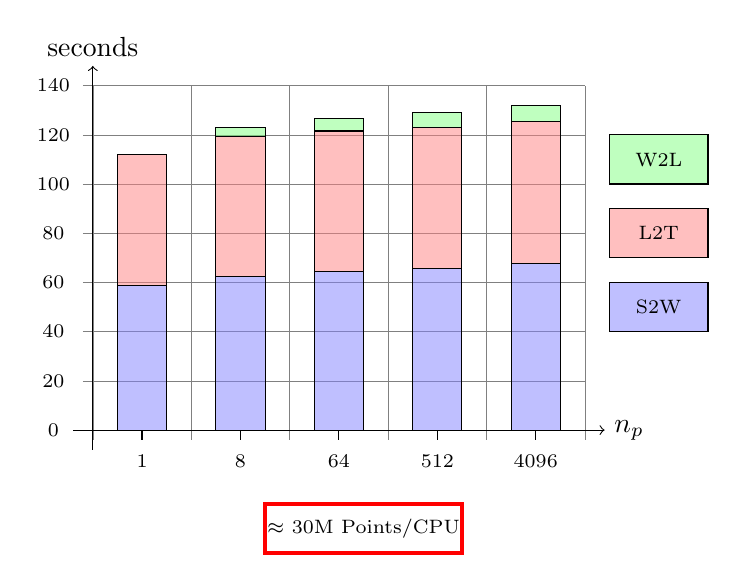
\begin{tikzpicture}[scale=1.25]

\draw[very thin, color=gray, xstep=1, ystep=0.5] (-0.1,-0.1) grid (5, 3.5);
\draw[->] (-0.2, 0) -- (5.2, 0) node[right] {$n_p$};
\draw[->] (0, -0.2) -- (0, 3.7) node[above] {seconds};

\newdimen\yscale

\yscale= 0.025 cm

\foreach \pos/\label in {0.5/1, 1.5/8, 2.5/64, 3.5/512, 4.5/4096} {
\draw (\pos,0) -- (\pos,-0.1) (\pos cm,-2.5ex) node [anchor=base,fill=white,inner sep=1pt]  {\scriptsize{\label}};
}

\foreach \label in {0, 20, ..., 140} {
 \draw (-0.4, \label\yscale) node {\scriptsize{\label}};
}

\draw[fill=blue!50, fill opacity=0.5] (4.5, 2.25) ++ (0.75, -1.25) rectangle +(1.0, 0.5);
\draw (4.5, 2.25) ++ (1.25, -1.0) node {\scriptsize{S2W}};

\draw[fill=red!50, fill opacity=0.5] (4.5, 1.75) ++ (0.75, 0.0) rectangle +(1.0, 0.5);
\draw (4.5, 1.75) ++ (1.25, 0.25) node {\scriptsize{L2T}};

\draw[fill=green!50, fill opacity=0.5] (4.5, 1.25) ++ (0.75, 1.25) rectangle +(1.0, 0.5);
\draw (4.5, 1.25) ++ (1.25, 1.5) node {\scriptsize{W2L}};

\draw[red, ultra thick] (1.75, -1.25) rectangle +(2.0, 0.5);
\draw (2.75, -1.0) node {\scriptsize{$\approx$ 30M Points/CPU}};

\newdimen\mypos
\newdimen\myoff

\foreach \pos/\vala/\valb/\valc/\vald/\vale/\valf in { 
0/58.75/53.36/0.0698/112.19/29.2M/$\frac{1}{16}$,
1/62.25/56.98/3.90/120.93/233.8M/$\frac{1}{64}$,
2/64.39/57.18/4.93/125.06/1.9B/$\frac{1}{256}$,
3/65.56/57.50/5.92/127.62/15.0B/$\frac{1}{1024}$,
4/67.53/57.75/6.59/131.65/119.7B/$\frac{1}{4096}$ } { 

\mypos=\pos cm
\advance \mypos by 0.5 cm

\advance \mypos by -0.25 cm

\myoff=0 cm

\draw[fill=blue!50, fill opacity=0.5] (\mypos, \myoff) rectangle +(0.5, \vala\yscale);
\advance \myoff by \vala\yscale

\draw[fill=red!50, fill opacity=0.5] (\mypos, \myoff) rectangle +(0.5, \valb\yscale);
\advance \myoff by \valb\yscale

\draw[fill=green!50, fill opacity=0.5] (\mypos, \myoff) rectangle +(0.5, \valc\yscale);

}

\end{tikzpicture}


	\end{center}
\caption{\label{f:isoUniform} Isogranular scalability for an uniform point distribution. For
 this experiment, we set $\epsilon = 10^{-6}$. The reported times for 
each component are the maximum values for that component across all the processors. The total wall-clock
time is reported in bold face.} \label{fig:uniform}
\end{figure}

{\em Example 2.} In this example, we consider a Gaussian random distribution of points in the unit cube. 
We present the weak scalability results in Figure \ref{fig:nonuniform}. 

\begin{figure}
	\begin{center}
	
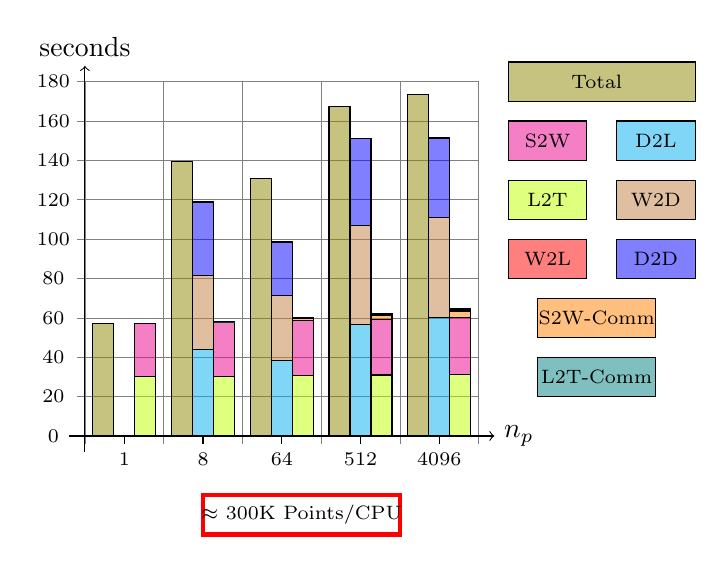
\begin{tikzpicture}[scale=1.0]

\draw[very thin, color=gray, xstep=1, ystep=0.5] (-0.1,-0.1) grid (5, 4.5);
\draw[->] (-0.2, 0) -- (5.2, 0) node[right] {$n_p$};
\draw[->] (0, -0.2) -- (0, 4.7) node[above] {seconds};

\newdimen\yscale

\yscale= 0.025 cm

\foreach \pos/\label in {0.5/1, 1.5/8, 2.5/64, 3.5/512, 4.5/4096} {
\draw (\pos,0) -- (\pos,-0.1) (\pos cm,-2.5ex) node [anchor=base,fill=white,inner sep=1pt]  {\scriptsize{\label}};
}

\foreach \label in {0, 20, ..., 180} {
 \draw (-0.4, \label\yscale) node {\scriptsize{\label}};
}


\draw[fill=olive, fill opacity=0.5] (5.375, 4.25) rectangle +(2.375, 0.5);
\draw (6.5, 4.5) node {\scriptsize{Total}};

\draw[fill=magenta, fill opacity=0.5] (5.375, 3.5) rectangle +(1.0, 0.5);
\draw (5.875, 3.75) node {\scriptsize{S2W}};

\draw[fill=lime, fill opacity=0.5] (5.375, 2.75) rectangle +(1.0, 0.5);
\draw (5.875, 3.0) node {\scriptsize{L2T}};

\draw[fill=red, fill opacity=0.5] (5.375, 2.0) rectangle +(1.0, 0.5);
\draw (5.875, 2.25) node {\scriptsize{W2L}};

\draw[fill=cyan, fill opacity=0.5] (6.75, 3.5) rectangle +(1.0, 0.5);
\draw (7.25, 3.75) node {\scriptsize{D2L}};

\draw[fill=brown, fill opacity=0.5] (6.75, 2.75) rectangle +(1.0, 0.5);
\draw (7.25, 3.0) node {\scriptsize{W2D}};

\draw[fill=blue, fill opacity=0.5] (6.75, 2.0) rectangle +(1.0, 0.5);
\draw (7.25, 2.25) node {\scriptsize{D2D}};

\draw[fill=orange, fill opacity=0.5] (5.75, 1.25) rectangle +(1.5, 0.5);
\draw (6.5, 1.5) node {\scriptsize{S2W-Comm}};

\draw[fill=teal, fill opacity=0.5] (5.75, 0.5) rectangle +(1.5, 0.5);
\draw (6.5, 0.75) node {\scriptsize{L2T-Comm}};

\draw[red, ultra thick] (1.5, -1.25) rectangle +(2.5, 0.5);
\draw (2.75, -1.0) node {\scriptsize{$\approx$ 300K Points/CPU}};


\newdimen\mypos
\newdimen\myoff

\foreach \pos/\vala/\valb/\valc/\vald/\vale/\valf/\valg/\valh/\vali/\valj/\valk/\vall/\valm in {
 0/0/0/0/30.07/27.18/0.0094/0.0045/0.014/57.28/827/0/283.7K/$\frac{1}{16}$,
 1/43.93/37.48/37.46/30.27/27.37/0.426/0.014/0.143/139.4/6666/6/2.3M/$\frac{1}{64}$,
 2/38.37/32.88/27.31/30.86/27.78/1.03/0.052/0.34/130.7/53929/126/18.5M/$\frac{1}{256}$,
 3/56.84/50.16/44.36/30.97/28.41/1.99/0.187/0.471/167.36/433226/880/148.9M/$\frac{1}{1024}$,
 4/60.18/50.65/40.56/31.08/29.24/3.18/0.567/0.924/173.42/3474244/7837/1.2B/$\frac{1}{4096}$
  } { 

\mypos=\pos cm
\advance \mypos by 0.5 cm

\advance \mypos by -0.4 cm
\myoff=0 cm

%Total

\draw[fill=olive, fill opacity=0.5] (\mypos, \myoff) rectangle +(0.266667, \vali\yscale);

%Direct

\advance \mypos by 0.266667 cm

\myoff=0 cm

\draw[fill=cyan, fill opacity=0.5] (\mypos, \myoff) rectangle +(0.266667, \vala\yscale);
\advance \myoff by \vala\yscale

\draw[fill=brown, fill opacity=0.5] (\mypos, \myoff) rectangle +(0.266667, \valb\yscale);
\advance \myoff by \valb\yscale

\draw[fill=blue, fill opacity=0.5] (\mypos, \myoff) rectangle +(0.266667, \valc\yscale);

%Expand

\advance \mypos by 0.266667 cm

\myoff=0 cm

\draw[fill=lime, fill opacity=0.5] (\mypos, \myoff) rectangle +(0.266667, \vald\yscale);
\advance \myoff by \vald\yscale

\draw[fill=magenta, fill opacity=0.5] (\mypos, \myoff) rectangle +(0.266667, \vale\yscale);
\advance \myoff by \vale\yscale

\draw[fill=orange, fill opacity=0.5] (\mypos, \myoff) rectangle +(0.266667, \valf\yscale);
\advance \myoff by \valf\yscale

\draw[fill=teal, fill opacity=0.5] (\mypos, \myoff) rectangle +(0.266667, \valg\yscale);
\advance \myoff by \valg\yscale

\draw[fill=red, fill opacity=0.5] (\mypos, \myoff) rectangle +(0.266667, \valh\yscale);

}

\end{tikzpicture}


	\end{center}
\caption{\label{f:isoGaussian} Isogranular scalability for a gaussian point distribution. For
 this experiment, we set $\epsilon = 10^{-3}$. The reported times for each component are the
 maximum values for that component across all the processors. The total wall-clock
time is reported in bold face.} \label{fig:nonuniform}
\end{figure}
